\documentclass{article}
\usepackage{asymptote}
\usepackage[utf8]{inputenc}
\usepackage{amssymb}
\usepackage{amsmath}
% \usepackage{amsfonts}
\usepackage{graphicx}
\newcommand{\Z}{\mathbb{Z}}
\newcommand{\R}{\mathbb{R}}

\DeclareMathOperator{\diag}{diag}
\DeclareMathOperator{\erf}{erf}

%\def\asydir{}
%\begin{asydef}

%\end{asydef}


\title{The Human Password Model}
\author{Carson Snart}
\date{December 2014}

\begin{document}

\maketitle

\section{Introduction}
hi.
\section{Multinomial Distribution}
Selecting independent samples (with repetition) from a discrete set of outcomes follows the multinomial distribution.

Specifically, select $N$ independent samples (with repetition) from a discrete set of possible outcomes $\left\{w_i\right\}_{i=1}^{\infty}$ with probabilities $p_i=P(w_i)$,  $\sum_{i=1}^{\infty} p_i = 1$.  Not considering order, this will result in $x_i \in Z_{0+}$ counts of outcome $w_i$, $\sum_{i=1}^\infty x_i = N$.  Note only finitely many $x_i$ can be non-zero.
The probability of such a sample is given by the multinomial distribution:
\begin{equation}
\label{eq:multinomial}
P_{\text{multinomial}}(x;p)={N!}\prod_{i=1}^{\infty} \frac{p_i^{x_i}}{x_i!} \,. 
\end{equation}
Since only finite number of $x_i$ are not zero, only a finite number of the factors in the product are not one.

The counts $x_i$ are not independent (they must sum to $N$), but if the probabilities are small, then the multinomial distribution can be treated as a product of independent Poisson distributions:
\begin{equation}
P_{\text{poisson}}(x;p) = \prod_{i=1}^{\infty} \frac{e^{-p_i} p_i^{x_i}}{x_i!} \,.
\end{equation}

\section{Stirling approximation}
\begin{equation}
n!=\Gamma(n+1) \approx S(n) = n^n e^{-n} \sqrt{\pi \left(2n+\frac{1}{3}\right)}
\end{equation}
Note the $+\frac{1}{3}$ is usually omitted, but including the term makes a better asymptotic approximation, and it matches 0!=1 much better than without this term.

\begin{figure}
  \caption{Stirling (modified) $S(n)$ (red) vs Stirling (unmodified blue) vs. $\Gamma(n+1)$ (green)}
  \centering
    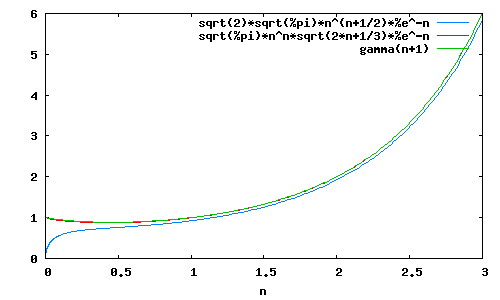
\includegraphics[width=1.0\textwidth]{img/stirling}
\end{figure}

\section{Luck}
In a large space, most outcomes will typically be improbable, so any outcome seems miraculous.  This is clearly nonsense; just a consequence of many improbable outcomes, so a suggested measure of luck is
\begin{equation}
\label{eq:luck}
L(w) = \sum_{P(w') > P(w)} P(w') + \frac{1}{2} \sum_{P(w') = P(w)} P(w') \,.
\end{equation}
In words, $L(w)$ is the fraction of the probability space more likely than $w$, plus $\frac{1}{2}$ the fraction of the probability space that is equally likely.  

For any fixed outcome $w$ and large independent sample $W=\left\{w_i\right\}_{i=1}^{n}$
\begin{itemize}
\item The fraction of outcomes which are more probable plus 1/2 the outcomes that are equally probable compared to $w$ is about $L(w)$.
\item The fraction of outcomes which are less probable plus 1/2 the outcomes that are equally probable compared to $w$ is about $1-L(w)$.
\item $L(w) \leq 1$, and $L(w)=1$ only if $P(w)=0$, so you must be perfectly lucky to get an impossible outcome.
\item If $L(w)$ is close to 1, then $P(w)$ is comparatively small, and most outcomes in $W$ would have a higher probability (you are lucky).  
\item If $L(w)$ is close to 0, then $P(w)$ is comparatively large, and most outcomes in $W$ would have a lower probability (you are unlucky).
\item The $f$ fraction of typical (neither lucky nor unlucky) outcomes would have luck in the range $\frac{1}{2} \pm \frac{1}{2}f$. 
\end{itemize}

Luck is a uniformizing mapping of the probability space to the unit interval.  Unlike a cumulative distribution, it makes a value choice on arranging the space from high-probability events through low probability events, which is consistent to with the natural sense of "luck" in everyday life.  For any finite set of probabilities,
\begin{align}
E(L) &= \frac{1}{2} \,, \\
E(L^2) &= \frac{1}{3} \,, \\
E(L^\alpha) &= \frac{1}{\alpha+1} + \epsilon\,,\alpha \geq 1 \text{ and } |{\epsilon}| \leq \frac{1}{24}k^2 \Delta^3 \,,\\
E(L \in [a,b]) &= (b-a)+2\Delta \,.
\end{align}
The error term in the last two estimates depend on $\Delta$, which is the largest constant probability distribution:
\begin{equation}
\Delta = \max_{w} \sum_{P(w')=P(w)} P(w')
\end{equation}

We are particularly interested in the luck of a given multinomial distribution (\ref{eq:multinomial}).  However, even for relatively modest values of $N$, the corresponding sum (\ref{eq:luck}) is intractable.

We instead consider the multivariate normal (Gaussian) distribution of a random variable $x \in R^n$ with mean $\mu$ and covariance $\sigma$:
\begin{align}
P_{\text{normal}}(x;\mu,\sigma) &= \frac{e^{-\frac{1}{2}(x-\mu)^T \sigma^{-1} (x-\mu)}}{\sqrt{(2\pi)^n \det{\sigma}}}  \,,\\
\intertext{where}
\mu_i &= E(x_i)\,,\\
\intertext{and}
\sigma_{ij} &= E((x_i-\mu_i)(x_j-\mu_j)) \,.
\end{align}

For the multinomial distribution ($N$ is the number of samples and $p_i$ is the probability of outcome $w_i$ and $x_i$ is the observed number of outcomes):
\begin{align}
\mu_i &= N p_i
\intertext{and}
\sigma_{ij}&=\begin{cases}
N p_i(1-p_i),& \text{if $i=j$} \\
-N p_i p_j,   & \text{if $i \neq j$}
\end{cases}
\end{align}
In matrix notation, $\mu=N p$ and $\sigma= N \cdot (\diag(p)-p p^{T})$.

Suppose an observation $x$ is made, how lucky is it?

\begin{equation}
L(x)=\int_{\Omega(x)} P_{\text{normal}}(x';\mu,\sigma) \,dx
\end{equation}
where 
\begin{align}
\Omega(x) &= \left\{ x' \in \R^n \middle| P_{\text{normal}}(x') > P_{\text{normal}}(x) \right\} \\
          &= \left\{ x' \in \R^n \middle| ||z(x')|| < ||z(x)||\,,\text{ where } z(x)=\sqrt{\sigma^{-1}} (x-\mu) \right\}
\end{align}
Note that, since in the continuous case the boundary $\partial \Omega(x)$ has zero volume the portion of equal probability is zero.

\begin{align}
L(x)&=\int_{\Omega(x)} P_{\text{normal}}(x';\mu,\sigma) \,dx' \\
\intertext{changing variables to $z=\sqrt{\sigma^{-1}} (x-\mu)$,}
    &=\int_{||z'||<||z||}  P_{\text{normal}}(z';0,I) \, dz' \\
\intertext{converting to spherical coordinates with $r_0 = ||\sqrt{\sigma^{-1}} (x-\mu)||$,}
    &=\frac{1}{\sqrt{(2\pi)^{n}}} \int_{0}^{r_0} \frac{n \pi^{n/2}}{\Gamma(\frac{n}{2}+1)} r^{n-1} e^{-\frac{1}{2} r^2} \, dr \\
    &=\frac{\gamma(n/2,r_0^2/2)}{\Gamma(n/2)}
\end{align}
The last form uses the lower incomplete gamma function, defined to be
\begin{equation}
\gamma(s,x) = \int_0^{x} t^{s-1} e^{-t} \, dt
\end{equation}
For any value of $n$, but particularly for large values, we find the following approximation to be very good ($r_0 = ||\sqrt{\sigma^{-1}} (x-\mu)||$):
\begin{equation}
L(x) \approx \frac{1}{2}\left[1+\erf(r_0-\sqrt{n-1/2})\right]
\end{equation}
\begin{figure}
  \caption{Exact (blue) vs approximate (red) likeliness for normal distribution for $n=1$, $10$, and $100$.}
  \centering
    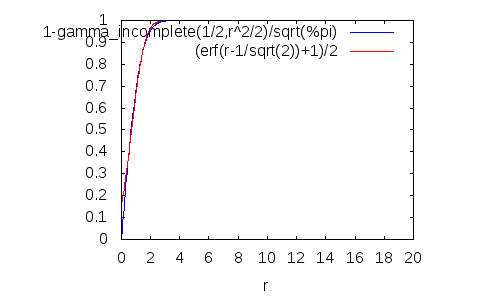
\includegraphics[width=0.75\textwidth]{img/luck1}
    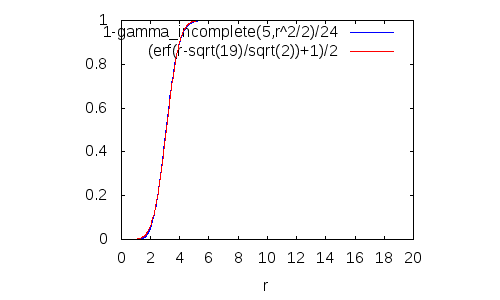
\includegraphics[width=0.75\textwidth]{img/luck10}
    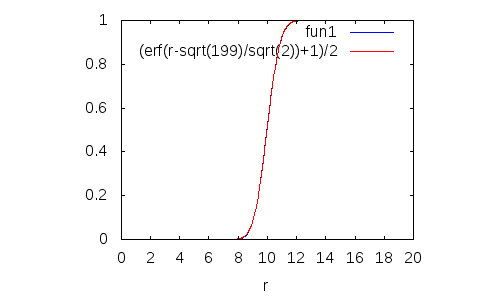
\includegraphics[width=0.75\textwidth]{img/luck100}
\end{figure}

Thus the luck of a multivariate normal closely approximates a single variable Gaussian, suggesting the following strong discriminator: 
\begin{equation}
\delta=1-|\erf(||\sigma^{-1}(x-\mu)||-\sqrt{n-1/2})|
\end{equation}
$\delta$ is how improbable (lucky or unlucky) the sample $x$ would be if it was actually sampled according to $P_{\text{normal}}(x;\mu,\sigma)$.

\subsection{Estimating luck.}
Computing the luck of an outcome directly is not always practical or feasible.  However, if a sample of the probability space is available, $W=\left\{w_i\right\}_{i=1}^{n}$, the luck of a given outcome can be estimated as:
\begin{equation}
L(w) \approx \ell(w) =  \sum_{P(w_i)>P(w)} \frac{1}{n} + \sum_{P(w_i) = P(w)} \frac{1}{2n}
\end{equation}
In the multinomial sample space for $W$, we have 
\begin{equation}
E(\ell(w))=L(w)\,,
\end{equation}
and
\begin{equation}
E((\ell(w)-L(w))^2)=\frac{L(w)\cdot(1-L(w))}{n} \,.
\end{equation}

Since $W$ follows a multinomial distribution (which is not necessarily normal).

\begin{figure}
\caption{A probabilistic automota.}
\begin{center}
\begin{asy}
import math;
import graph;

size(4cm,0);


pair p0=(2,1);
pair p1=(2,3);
pair pa=(3,2);
pair pb=(1,2);

real r=0.30;

draw(circle(p0,r)); label("$0$",p0);
draw(circle(p1,r)); label("$1$",p1);
draw(circle(pa,r)); label("$[a]$,pa);
draw(circle(pb,r)); label("$[b]$,pb);
\end{asy}
\end{center}
\label{fig:pa}
\end{figure}


\end{document}
